\documentclass[aspectratio=169,10pt]{beamer}
% Message & body slide style. Compile with xelatex.
\usepackage{xeCJK}
\setCJKmainfont[BoldFont={Hiragino Sans W6}]{Hiragino Sans W3}
\setCJKsansfont[BoldFont={Hiragino Sans W6}]{Hiragino Sans W3}
\setmainfont{Helvetica Neue}
\setsansfont{Helvetica Neue}
% circled digits and arrows must come from the Japanese font
\xeCJKDeclareCharClass{FullLeft}{"2460->"2473}
\xeCJKDeclareCharClass{CJK}{"2192, "2190, "2460->"2473}
\usepackage{graphicx,booktabs,tabularx,array,colortbl,xcolor,tikz,multirow}
\usetikzlibrary{arrows.meta,positioning,shapes.misc}

\definecolor{ink}{HTML}{1A202C}
\definecolor{muted}{HTML}{6B6B6B}
\definecolor{accent}{HTML}{2B6CB0}
\definecolor{accent2}{HTML}{C05621}
\definecolor{good}{HTML}{2F855A}
\definecolor{bad}{HTML}{C53030}
\definecolor{soft}{HTML}{F2F5F9}
\definecolor{rule}{HTML}{D5DCE4}

\setbeamertemplate{navigation symbols}{}
\setbeamercolor{normal text}{fg=ink}
\setbeamerfont{normal text}{size=\small}
\setbeamercolor{structure}{fg=accent}
\setbeamertemplate{itemize item}{\color{accent}\raisebox{0.15ex}{\scriptsize$\blacksquare$}}
\setbeamertemplate{itemize subitem}{\color{muted}--}
\setlength{\leftmargini}{1.1em}

% --- frame title = section tag (small) + message (1-2 sentences) ---
\newcommand{\slidetag}{}
\newcommand{\settag}[1]{\renewcommand{\slidetag}{#1}}
\setbeamertemplate{frametitle}{%
  \vspace{0.35cm}%
  \begin{minipage}{\textwidth}
    {\color{accent}\scriptsize\bfseries\slidetag}\par\vspace{0.12cm}
    {\color{ink}\large\bfseries\insertframetitle\par}
    \vspace{0.18cm}{\color{rule}\rule{\textwidth}{0.8pt}}
  \end{minipage}}
\setbeamertemplate{footline}{%
  \leavevmode\hbox to\paperwidth{\hspace{0.45cm}{\color{muted}\tiny ETT Oil-Temperature Forecasting PoC}\hfill
  {\color{muted}\tiny\insertframenumber}\hspace{0.45cm}}\vspace{0.22cm}}

\newcommand{\source}[1]{\vfill{\color{muted}\tiny #1}}
\newcommand{\hl}[1]{{\color{accent}\bfseries #1}}
\newcommand{\hlb}[1]{{\color{bad}\bfseries #1}}
\newcommand{\hlg}[1]{{\color{good}\bfseries #1}}
\newcommand{\fig}[2][]{\includegraphics[#1]{../outputs/figures/#2.png}}
\newcommand{\softbox}[2]{\begin{beamercolorbox}[sep=6pt,rounded=false]{soft}#2\end{beamercolorbox}}
\setbeamercolor{soft}{bg=soft,fg=ink}
\newcommand{\kpi}[3]{% value, label, color
  \begin{minipage}[t]{0.23\textwidth}\centering
    {\color{#3}\fontsize{20}{22}\selectfont\bfseries #1}\par\vspace{0.1cm}
    {\scriptsize\color{muted}#2}
  \end{minipage}}

\graphicspath{{../outputs/figures/}}

\begin{document}

% ------------------------------------------------------------------ title
{\setbeamertemplate{footline}{}
\begin{frame}[plain]
  \vspace{1.2cm}
  {\color{accent}\small\bfseries 技術検証（PoC）報告書}\par\vspace{0.3cm}
  {\color{ink}\LARGE\bfseries 変圧器油温の24時間先予測による\\[0.15cm]予防保全への適用可能性}\par\vspace{0.4cm}
  {\color{muted}\normalsize 公開ベンチマーク ETT データセット（ETTh1 / ETTh2）を用いた検証}\par
  \vfill
  {\color{rule}\rule{\textwidth}{0.8pt}}\par\vspace{0.15cm}
  {\small Pyii Phyo Maung}\hfill{\small\color{muted}2026年11月}
  \vspace{0.6cm}
\end{frame}}

% ------------------------------------------------------------------ 1 summary
\settag{エグゼクティブサマリー}
\begin{frame}{負荷計画を用いた予測アラートにより、過熱の87\%を約21時間前に予告できる。ただし精度向上は誤差5〜9\%に留まり、本格導入には外気温データが必要}
  \kpi{−9.1\%}{24h先予測誤差（ETTh1）\\「現在値維持」比}{accent}\hfill
  \kpi{87\%}{過熱開始の事前警告率\\（ETTh2、誤報 月11時間）}{good}\hfill
  \kpi{約21h}{警告のリードタイム\\（中央値）}{accent2}\hfill
  \kpi{0h}{現行の閾値監視の\\リードタイム}{bad}
  \vspace{0.2cm}
  \begin{columns}[T]
    \begin{column}{0.49\textwidth}
      \softbox{}{\scriptsize\textbf{分かったこと}
      \begin{itemize}\setlength{\itemsep}{1pt}
        \item 油温は慣性が強く24h先の改善は5〜9\%に留まるが、\hl{3〜6時間先なら誤差を13〜53\%削減}できる
        \item 最良は物理に基づく特徴量＋線形モデル。GBM・LSTM等の複雑なモデルは上回らなかった
        \item 価値は精度よりも「警告の先行時間」にある。翌日の負荷計画が鍵
        \item 予測区間はそのままでは過小（被覆77〜84\%）。コンフォーマル補正で90\%に校正
      \end{itemize}}
    \end{column}
    \begin{column}{0.49\textwidth}
      \softbox{}{\scriptsize\textbf{提言}
      \begin{itemize}\setlength{\itemsep}{1pt}
        \item \hl{外気温データの連携}を最優先（日内変動の主因と推定。異常検知の前提条件）
        \item 実際の警報温度・故障履歴を共有いただき、\hl{3か月のシャドー運用}で警告ルールを検証
        \item 公開データにはセンサ固着・欠測補完の痕跡があり、\hl{データ品質監視}は即日導入可能
      \end{itemize}}
    \end{column}
  \end{columns}
  \source{評価：2017年7月〜2018年6月の12か月、月次ローリング検証。警告率は過熱開始15件に基づく参考値。}
\end{frame}

% ------------------------------------------------------------------ 2 scope
\settag{検証の問いと前提}
\begin{frame}{「24時間前に過熱を予告できるか」を問いとし、翌日の負荷計画を使う予測（C）と使わない予測（B）を比較した}
  \begin{columns}[T]
    \begin{column}{0.56\textwidth}
      \centering
      \begin{tikzpicture}[x=0.62cm,y=0.62cm,font=\scriptsize]
        \draw[->,thick,muted] (0,0) -- (12.5,0) node[right]{時刻};
        \draw[thick] (6,-0.2) -- (6,0.2) node[above=2pt]{\textbf{t}（予測時点）};
        \draw[thick] (12,-0.2) -- (12,0.2) node[above=2pt]{\textbf{T = t+24h}};
        \fill[accent!25] (0,-1.1) rectangle (6,-0.5);
        \node at (3,-0.8) {実測：油温・負荷（過去）};
        \fill[accent2!25] (6,-1.9) rectangle (12,-1.3);
        \node at (9,-1.6) {翌日の負荷計画（Cのみ）};
        \fill[good!25] (6,-2.7) rectangle (12,-2.1);
        \node at (9,-2.4) {カレンダー（時刻・季節）};
        \node[draw=bad,thick,circle,inner sep=1.5pt,fill=white] at (12,-3.3) {\textbf{?}};
        \node[below=3pt] at (12,-3.7) {油温 OT(T)};
      \end{tikzpicture}
    \end{column}
    \begin{column}{0.42\textwidth}
      \footnotesize
      \begin{itemize}\setlength{\itemsep}{3pt}
        \item \textbf{予測対象}：24時間後の油温。保全準備（負荷調整・巡視）に必要な先行時間として設定
        \item \textbf{B（厳密予測）}：時点tまでの実測のみ
        \item \textbf{C（計画活用）}：課題で許容される「t=Tの特徴量」を\hl{翌日の負荷計画}として利用。計画誤差の影響も検証（p.14）
        \item \textbf{価値の定義}：精度（MAE）に加え、過熱を\hl{何時間前に、何回の誤報で}予告できるか
        \item 実際の警報温度は未提供のため、\hlb{開発期間の油温95パーセンタイル}を代理警報値とした
      \end{itemize}
    \end{column}
  \end{columns}
  \source{OT：油温（Oil Temperature）。負荷6系統（HUFL等）はETTの公開定義に従う。ETTm1/m2は同じ変圧器の15分値（毎正時の値はETTh1/h2と一致）。24時間先の判断には1時間解像度で十分と仮定し、時間データを使用。}
\end{frame}

% ------------------------------------------------------------------ 3 data quality
\settag{EDA ① データ品質}
\begin{frame}{公開データには毎月31日の全項目凍結や最長43日のセンサ固着があり、除外しなければ精度評価そのものが歪む}
  \begin{columns}[T]
    \begin{column}{0.62\textwidth}
      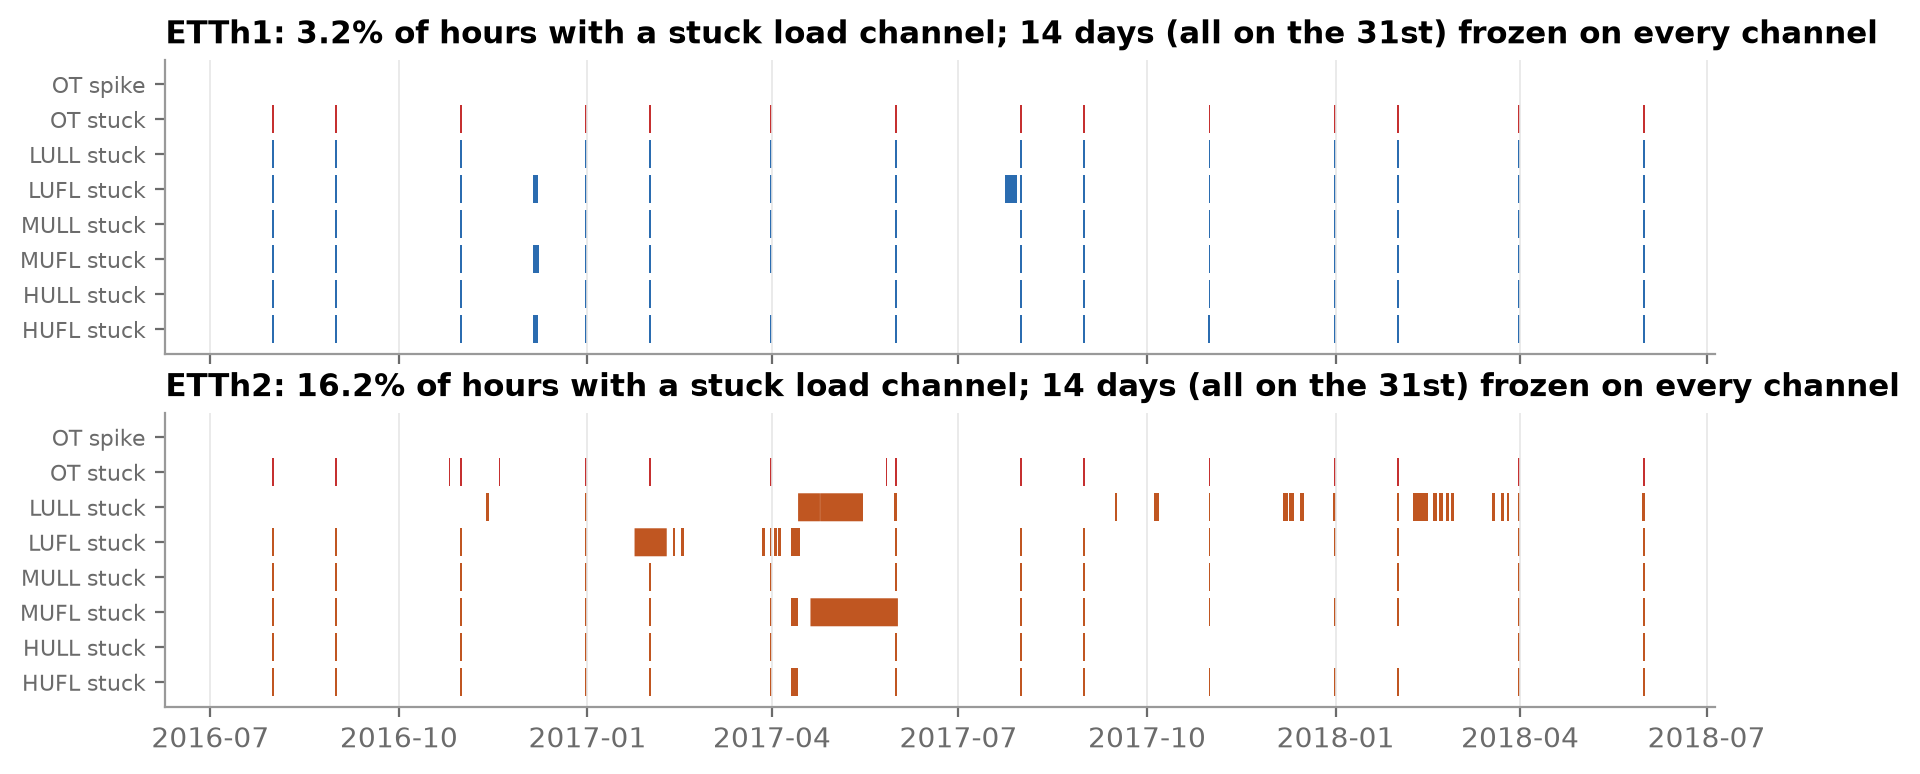
\includegraphics[width=\textwidth]{eda_data_quality}
    \end{column}
    \begin{column}{0.36\textwidth}
      \scriptsize
      \begin{itemize}\setlength{\itemsep}{2pt}
        \item \textbf{31日の凍結}：両変圧器とも\hl{毎月31日の24時間}が全7項目で同一値。収集・補完処理の痕跡と判断（各14日）
        \item \textbf{センサ固着}：ETTh2のMUFLが\hl{1,025時間（43日）}一定値。固着時間はETTh1 3.2\%、ETTh2 16.2\%
        \item \textbf{スパイク}：1時間で −20℃→+23℃ の往復（ETTh2）
        \item \textbf{整合性}：高圧側負荷＝中圧＋低圧の関係がETTh1では成立（r=0.99）、ETTh2では不成立（r=0.48）
      \end{itemize}
      \vspace{0.1cm}
      \softbox{}{\scriptsize\textbf{対応}：異常な目的値は学習・評価から除外。入力センサの固着を検知した場合は「現在値維持」に自動切替（運用時と同じ規則、過去データのみで判定）}
    \end{column}
  \end{columns}
  \source{固着：同一値が24時間以上継続（無効負荷のゼロは除く）。スパイク：前後5時間の中央値から6℃以上の乖離。}
\end{frame}

% ------------------------------------------------------------------ 4 drivers
\settag{EDA ② 温度変動の要因}
\begin{frame}{油温の日内ピーク（15〜16時）は負荷のピーク（0時・21時）と一致せず、日内変動の主因は未計測の外気温と考えられる}
  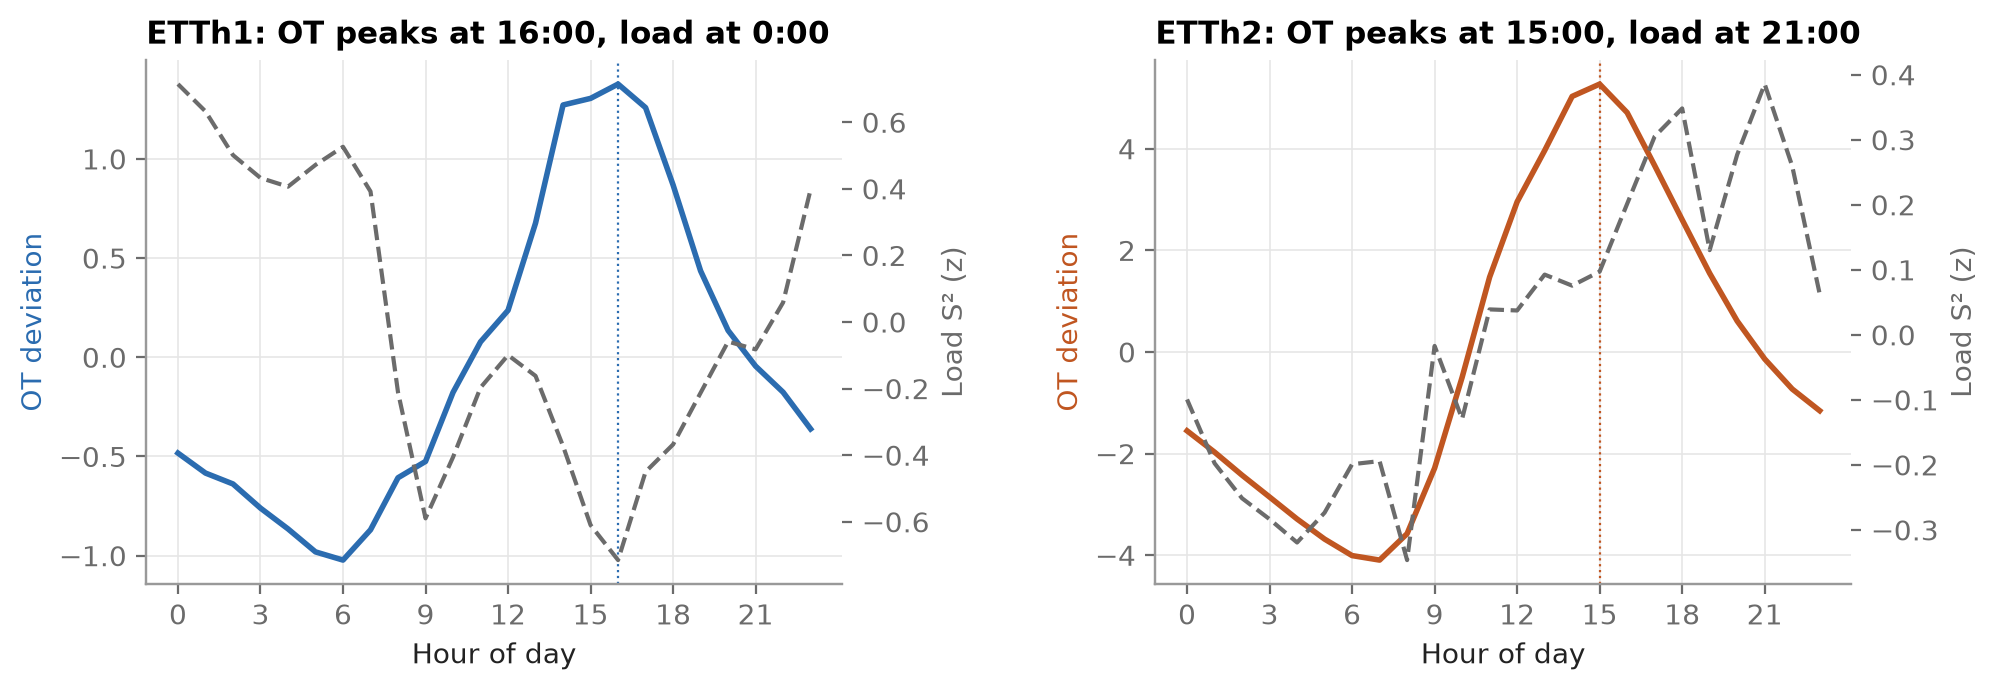
\includegraphics[width=\textwidth,height=3.9cm,keepaspectratio]{eda_daily_profile}
  \vspace{0.1cm}
  \begin{columns}[T]
    \begin{column}{0.49\textwidth}\scriptsize
      \begin{itemize}
        \item 油温と負荷の相関は弱い（季節成分除去後 r≈0.22）
        \item 負荷の効果は\hl{時間遅れ}を伴う。ETTh1は半減期18時間の平滑化負荷と最も相関し、熱容量の大きさを示唆
      \end{itemize}
    \end{column}
    \begin{column}{0.49\textwidth}\scriptsize
      \begin{itemize}
        \item 示唆：\hl{外気温を持たないことが本データ最大の制約}。モデルは時刻・季節の周期で代用するしかない
        \item 設計への反映：負荷は電流²に比例する発熱（S²=有効²+無効²）とし、複数の時定数で平滑化（IEC 60076-7）
      \end{itemize}
    \end{column}
  \end{columns}
  \source{季節成分は30日中心移動平均で除去（記述目的のみ。モデルには使用していない）。}
\end{frame}

% ------------------------------------------------------------------ 5 inertia & drift
\settag{EDA ③ 慣性と年次変化}
\begin{frame}{油温は慣性が強く1時間先なら「現在値」で十分だが、ETTh1は評価年に平均7.7℃低下しており、年をまたぐ頑健性が必要}
  \begin{columns}[T]
    \begin{column}{0.60\textwidth}
      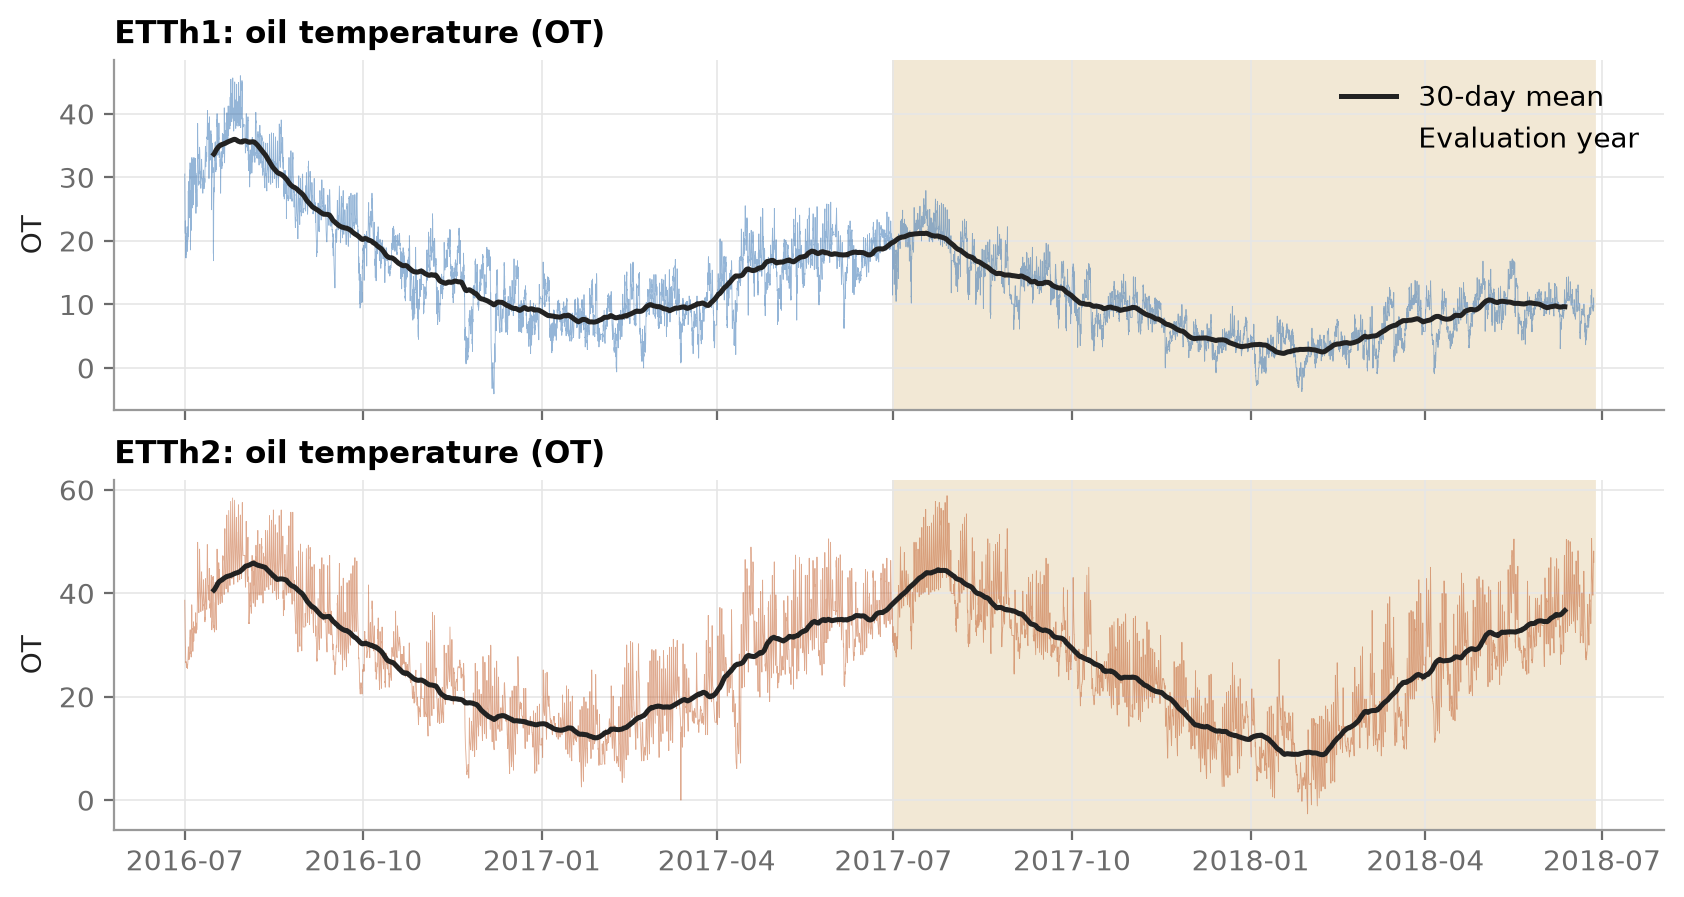
\includegraphics[width=\textwidth,height=4.0cm,keepaspectratio]{eda_ot_overview}
    \end{column}
    \begin{column}{0.38\textwidth}
      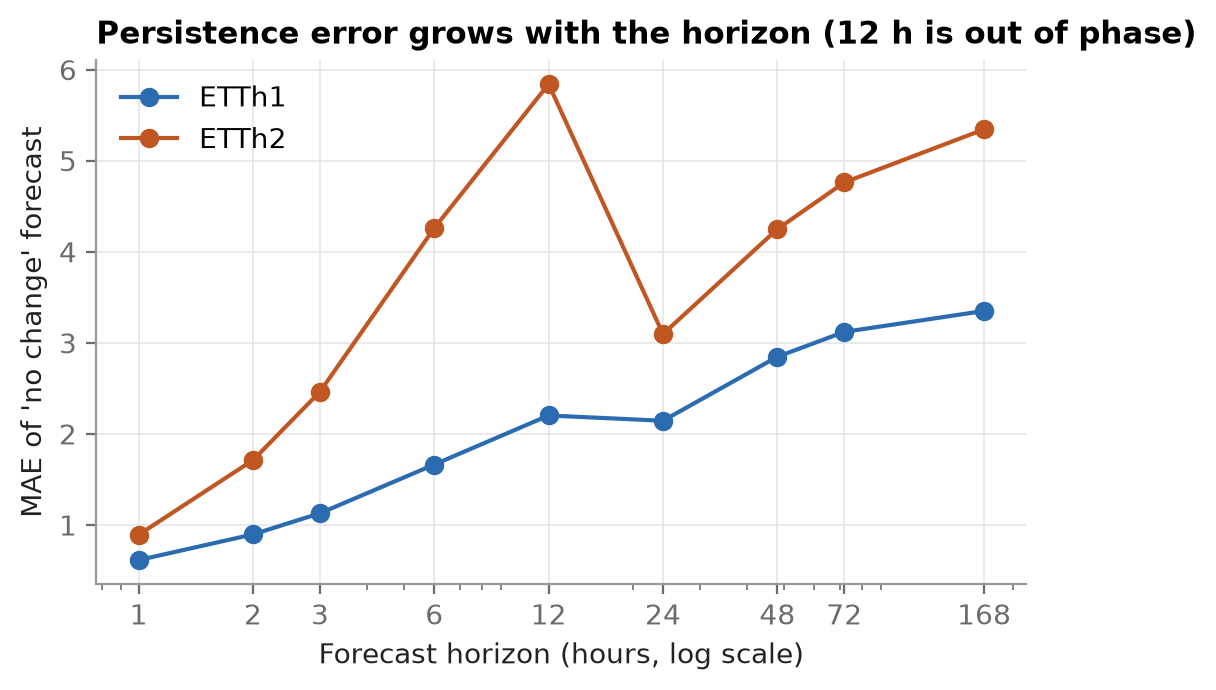
\includegraphics[width=\textwidth,height=4.0cm,keepaspectratio]{eda_persistence_horizon}
    \end{column}
  \end{columns}
  \vspace{0.05cm}
  \scriptsize
  \begin{itemize}\setlength{\itemsep}{1pt}
    \item 24時間後との自己相関は0.94。「現在値維持」の誤差は1時間先0.6℃、24時間先2.1℃（ETTh1）。\hl{価値が出るのは数時間〜1日先}
    \item ETTh1の評価年は前年より平均7.7℃低く、最高27.9℃と前年の代理警報値（35.2℃）に一度も届かない。\hlb{過去の水準を外挿できないモデルは劣化する}
  \end{itemize}
\end{frame}

% ------------------------------------------------------------------ 6 approach
\settag{アプローチと設計上の意思決定}
\begin{frame}{EDAを踏まえ、物理に基づく特徴量・温度「変化量」の予測・時系列ロール検証という、単純で頑健な設計を選んだ}
  \scriptsize
  \renewcommand{\arraystretch}{1.25}
  \begin{tabularx}{\textwidth}{>{\bfseries}p{3.0cm} X X}
    \toprule
    設計判断 & 内容 & 根拠 \\
    \midrule
    変化量を予測 & OT(T)−OT(t) を学習し、現在値に加算 & 年次の水準変化（p.6）。木モデルは学習範囲外を外挿できない \\
    物理特徴量 & 電流²に相当するS²、時定数3/12/48hの平滑化、熱モデルの時定数推定 & IEC 60076-7 の一次遅れ熱モデル。負荷影響の時間遅れ（p.5） \\
    強い基準との比較 & 「現在値維持」比のスキルとDiebold–Mariano検定 & 慣性が強い系列では単純予測が強い（Cui et al. 2021、Hewamalage et al. 2023） \\
    ロール検証 & 12か月×月次で再学習、全季節を評価。調整は開発期間のみ & 単一の春季テストでは季節依存の結論になる \\
    データ品質の自動処理 & 固着・スパイクを過去データのみで検知し、現在値予測へ切替 & p.4の欠陥が運用でも起こりうる \\
    区間の校正 & 分位点回帰＋コンフォーマル補正（CQR） & 区間の過小被覆が既知の課題（Tembo et al. 2025） \\
    \bottomrule
  \end{tabularx}
  \source{比較モデル：物理（グレーボックス）、Ridge、GBM（3変種）、物理＋GBMハイブリッド、MLP、生ウィンドウ線形（DLinear型）、LSTM、アンサンブル。詳細は付録。}
\end{frame}

% ------------------------------------------------------------------ 7 protocol
\settag{評価方法}
\begin{frame}{評価は「未来を一切見ない」ことを徹底し、12か月の月次ロール検証で全季節の汎化性能を測った}
  \centering
  \begin{tikzpicture}[x=0.52cm,y=0.42cm,font=\scriptsize]
    \foreach \i in {0,...,23} { \draw[rule] (\i,0.6) -- (\i,0.8); }
    \node[above] at (0,0.8) {2016-07};
    \node[above] at (24,0.8) {2018-06};
    \fill[muted!30] (0,-0.2) rectangle (8,0.3); \node at (4,0.05) {学習（調整用）};
    \fill[accent2!40] (8,-0.2) rectangle (12,0.3); \node at (10,0.05) {検証};
    \node[left] at (-0.2,0.05) {ハイパラ調整};
    \foreach \k/\y in {0/-1.0,1/-1.7,2/-2.4} {
      \fill[accent!35] (0,\y-0.25) rectangle (12+\k,\y+0.25);
      \fill[good!60] (12+\k,\y-0.25) rectangle (13+\k,\y+0.25);
    }
    \node at (14.5,-1.7) {$\cdots$};
    \fill[accent!35] (0,-3.65) rectangle (23,-3.15); \fill[good!60] (23,-3.65) rectangle (24,-3.15);
    \node[left] at (-0.2,-2.3) {評価（12分割）};
    \fill[accent!35] (2,-4.7) rectangle (3,-4.3); \node[right] at (3.1,-4.5) {学習（拡張窓）};
    \fill[good!60] (8,-4.7) rectangle (9,-4.3); \node[right] at (9.1,-4.5) {テスト月};
  \end{tikzpicture}
  \vspace{0.25cm}
  \begin{columns}[T]
    \begin{column}{0.32\textwidth}\footnotesize
      \textbf{リーク防止}
      \begin{itemize}
        \item 標準化・特徴量・閾値はすべて学習期間内で計算
        \item 分割は予測対象時刻で行う
      \end{itemize}
    \end{column}
    \begin{column}{0.32\textwidth}\footnotesize
      \textbf{指標}
      \begin{itemize}
        \item MAE・RMSE、「現在値維持」比スキル
        \item 油温が0℃付近を通るためMAPEは不使用
      \end{itemize}
    \end{column}
    \begin{column}{0.32\textwidth}\footnotesize
      \textbf{有意性}
      \begin{itemize}
        \item Diebold–Mariano検定（24h重複予測の自己相関をHAC分散で補正）
      \end{itemize}
    \end{column}
  \end{columns}
  \source{参考：Tashman (2000)、Hewamalage, Ackermann \& Bergmeir (2023)、Diebold \& Mariano (1995)、Harvey et al. (1997)}
\end{frame}

% ------------------------------------------------------------------ 8 accuracy
\settag{結果 ① 予測精度}
\begin{frame}{負荷計画を用いた線形モデルが最良で、24時間先の誤差を「現在値維持」比9.1\%（ETTh1）・4.8\%（ETTh2）削減した}
  \centering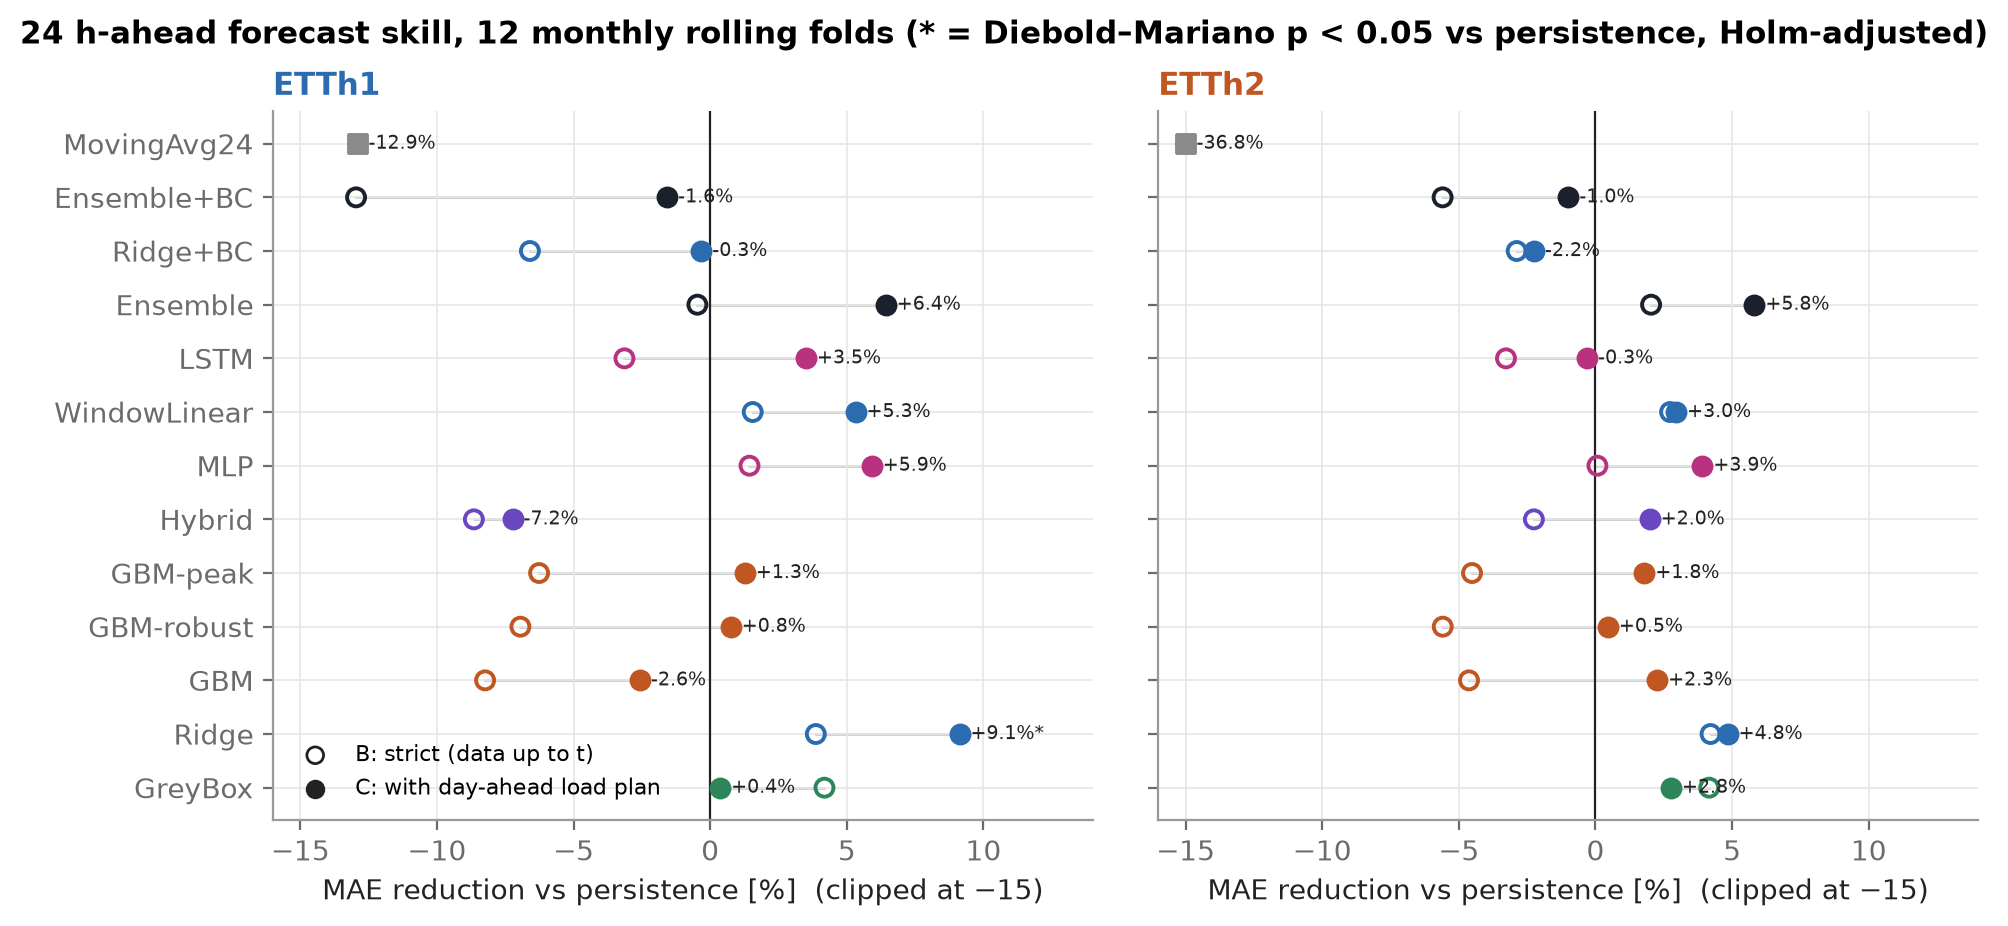
\includegraphics[width=\textwidth,height=4.9cm,keepaspectratio]{res_skill}\par\raggedright
  \scriptsize
  \begin{itemize}\setlength{\itemsep}{1pt}
    \item MAE：ETTh1 1.76→\hl{1.60℃}、ETTh2 3.25→\hl{3.09℃}（いずれも p<0.01）。等重みアンサンブル（C）は 6.1\% / 5.1\% で次点
    \item \hl{負荷計画（C）}は線形・木・アンサンブルで一貫して改善（ETTh1のRidgeで3.8\%→9.1\%）。一方、物理モデル単体は両変電所で悪化し、LSTMは変電所により逆の結果。計画情報の活かし方はモデル依存
  \end{itemize}
\end{frame}

% ------------------------------------------------------------------ 9 complexity
\settag{結果 ② モデルの複雑さ}
\begin{frame}{複雑なモデルほど良いわけではなく、GBM・LSTM・MLPは年次ドリフトの下で線形モデルを上回れなかった}
  \scriptsize
  \renewcommand{\arraystretch}{1.15}
  \begin{tabularx}{\textwidth}{>{\bfseries}p{4.2cm} c c X}
    \toprule
    手法（C：計画あり） & ETTh1 & ETTh2 & 解釈 \\
    \midrule
    Ridge（物理特徴量） & \hlg{+9.1\%*} & \hlg{+4.8\%*} & 最良。少数パラメータで外挿に強い \\
    アンサンブル（Ridge+GBM+Hybrid） & +6.1\%* & \hlg{+5.1\%*} & 安定。ETTh2で最良だが差は小 \\
    生ウィンドウ線形（DLinear型） & +5.3\%* & +2.9\% & 特徴量設計なしでも健闘（Zeng et al. 2023と整合） \\
    LSTM（生系列） & +3.5\% & −2.7\% & 系列モデルの優位性は確認できず \\
    GBM／頑健化GBM／ピーク重視GBM & −0.5〜+1.8\% & −0.7〜+4.1\% & 計画なし（B）では −5〜−12\%。水準の変化に弱い \\
    物理＋GBMハイブリッド & −7.9\%* & +1.9\% & 物理モデルの誤差を学習しきれず \\
    MLP & −45\%* & −17\%* & 過学習。データ量に対して不安定 \\
    直近7日の誤差による補正（+BC） & 悪化 & 悪化 & 誤差は持続的な偏りでなく天候由来の変動 \\
    \bottomrule
  \end{tabularx}
  \vspace{0.15cm}
  \softbox{}{\scriptsize\textbf{示唆}：精度の上限を決めているのはモデルの表現力ではなく\hl{入力情報（外気温の欠如）}。モデルを複雑にするより、データを追加する方が効果的と判断した。}
  \source{数値は24時間先MAEの「現在値維持」比削減率。* は Diebold–Mariano 検定 p<0.05。}
\end{frame}

% ------------------------------------------------------------------ 10 horizons
\settag{結果 ③ 予測の先行時間}
\begin{frame}{予測の価値は数時間〜半日先で最大（誤差を最大22〜53\%削減）となり、24時間先では5〜9\%に縮むため、用途で使い分けるべき}
  \centering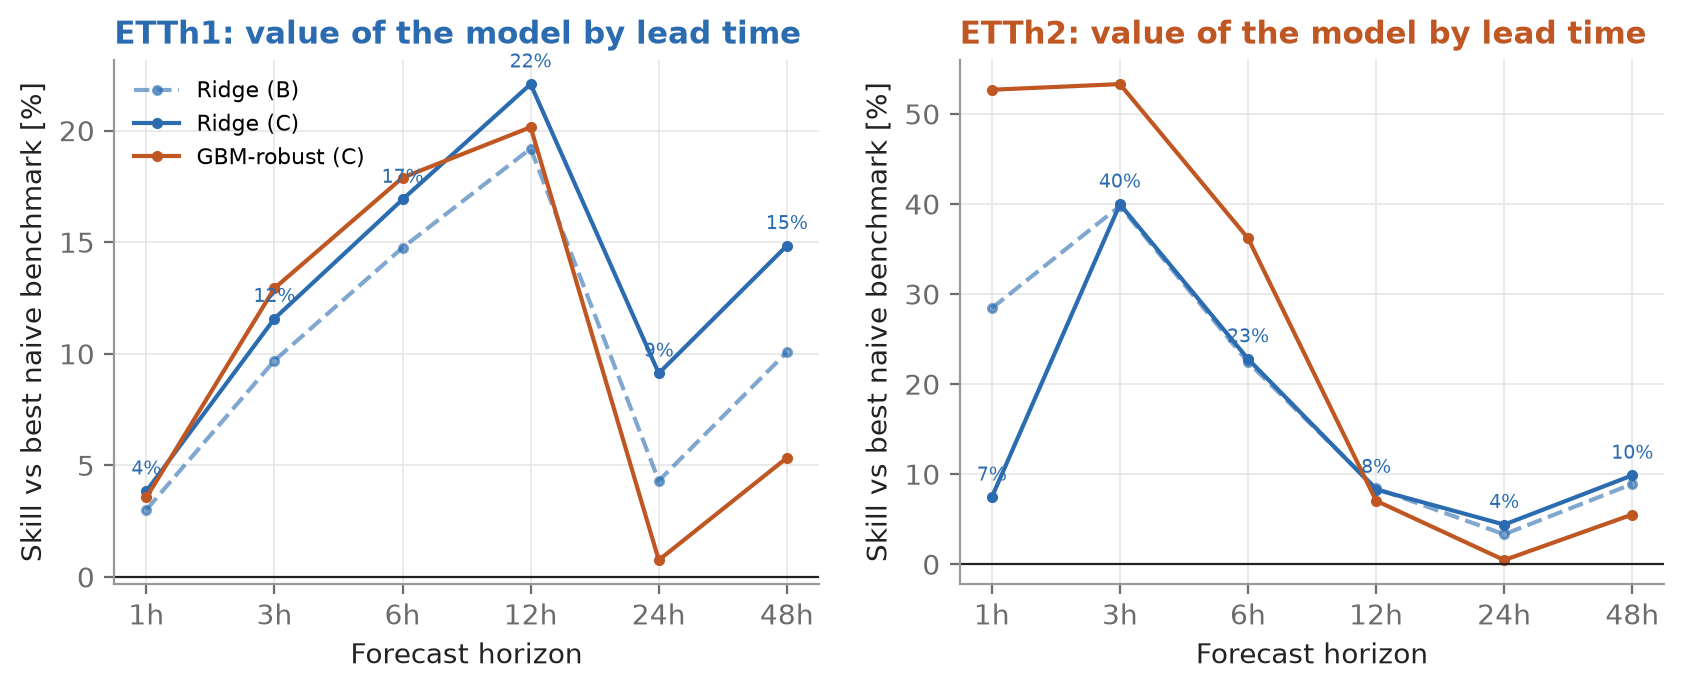
\includegraphics[width=\textwidth,height=3.7cm,keepaspectratio]{res_horizons}\par\raggedright
  \scriptsize
  \begin{itemize}\setlength{\itemsep}{1pt}
    \item \textbf{1〜6時間先}：頑健化GBMが最良。ETTh2で1h・3h先とも53\%、6h先で36\%削減。日内の加熱パターンを学習できている
    \item \textbf{12〜48時間先}：計画あり線形モデル（C）が最良。ETTh1は12h先で22\%と最大。ETTh2の12h先は「前日同時刻」が強く、改善は8\%に留まる
    \item \hl{使い分けの提案}：〜6h先＝負荷配分・冷却運転の判断、24h先＝巡視・保全計画の判断（警告はp.12）
  \end{itemize}
  \source{基準：「現在値維持」と「前日同時刻」のうち誤差の小さい方。同一の12か月ロール検証。}
\end{frame}

% ------------------------------------------------------------------ 11 alerts
\settag{業務価値 ① 過熱の事前警告}
\begin{frame}{警告の余裕幅を4℃とすれば、過熱開始の87\%を約21時間前に予告でき、誤報は月約11時間に抑えられる}
  \begin{columns}[T]
    \begin{column}{0.50\textwidth}
      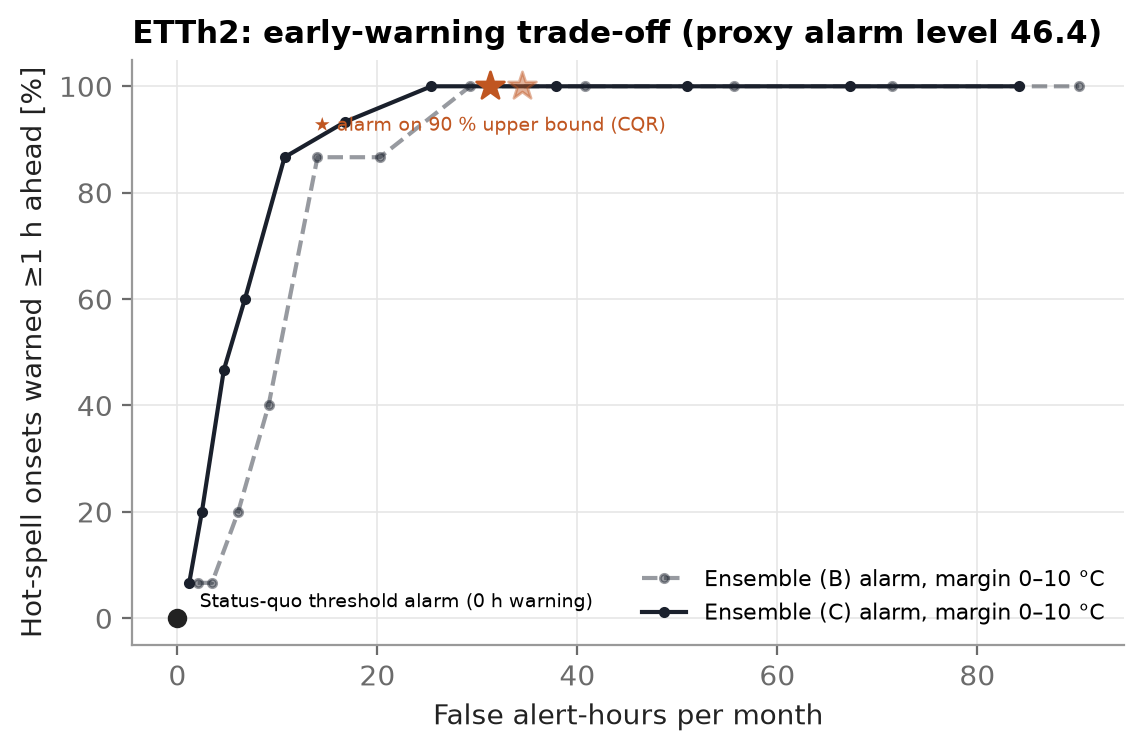
\includegraphics[width=\textwidth]{res_alert_tradeoff}
    \end{column}
    \begin{column}{0.48\textwidth}
      \scriptsize
      \renewcommand{\arraystretch}{1.2}
      \begin{tabular}{l c c}
        \toprule
        警告方式 & 事前警告率 & 誤報（時間/月） \\
        \midrule
        現行：閾値監視 & 0\% & -- \\
        予測（B）＋余裕4℃ & 87\% & 14.0 \\
        \textbf{予測（C）＋余裕4℃} & \hlg{87\%} & \hlg{10.7} \\
        予測（C）＋余裕3℃ & 60\% & 6.8 \\
        90\%区間の上限 & 100\% & 31.2 \\
        \bottomrule
      \end{tabular}
      \vspace{0.2cm}
      \begin{itemize}\setlength{\itemsep}{2pt}
        \item 余裕幅は\hl{運用者が選ぶつまみ}。誤報コストと見逃しコストで決める
        \item 負荷計画は同じ検知率を\hl{少ない誤報}で実現する
        \item ETTh1は評価年に代理警報値へ一度も達せず、評価対象外
      \end{itemize}
    \end{column}
  \end{columns}
  \source{ETTh2、過熱開始＝24時間以上の平常後に代理警報値（46.4、開発期間95パーセンタイル）を超えた時点、計15件。少数のため参考値。}
\end{frame}

% ------------------------------------------------------------------ 12 uncertainty
\settag{業務価値 ② 不確実性の提示}
\begin{frame}{分位点回帰の「90\%区間」は実際には77〜84\%しか当たらなかったが、コンフォーマル補正で90\%に校正できた}
  \begin{columns}[T]
    \begin{column}{0.62\textwidth}
      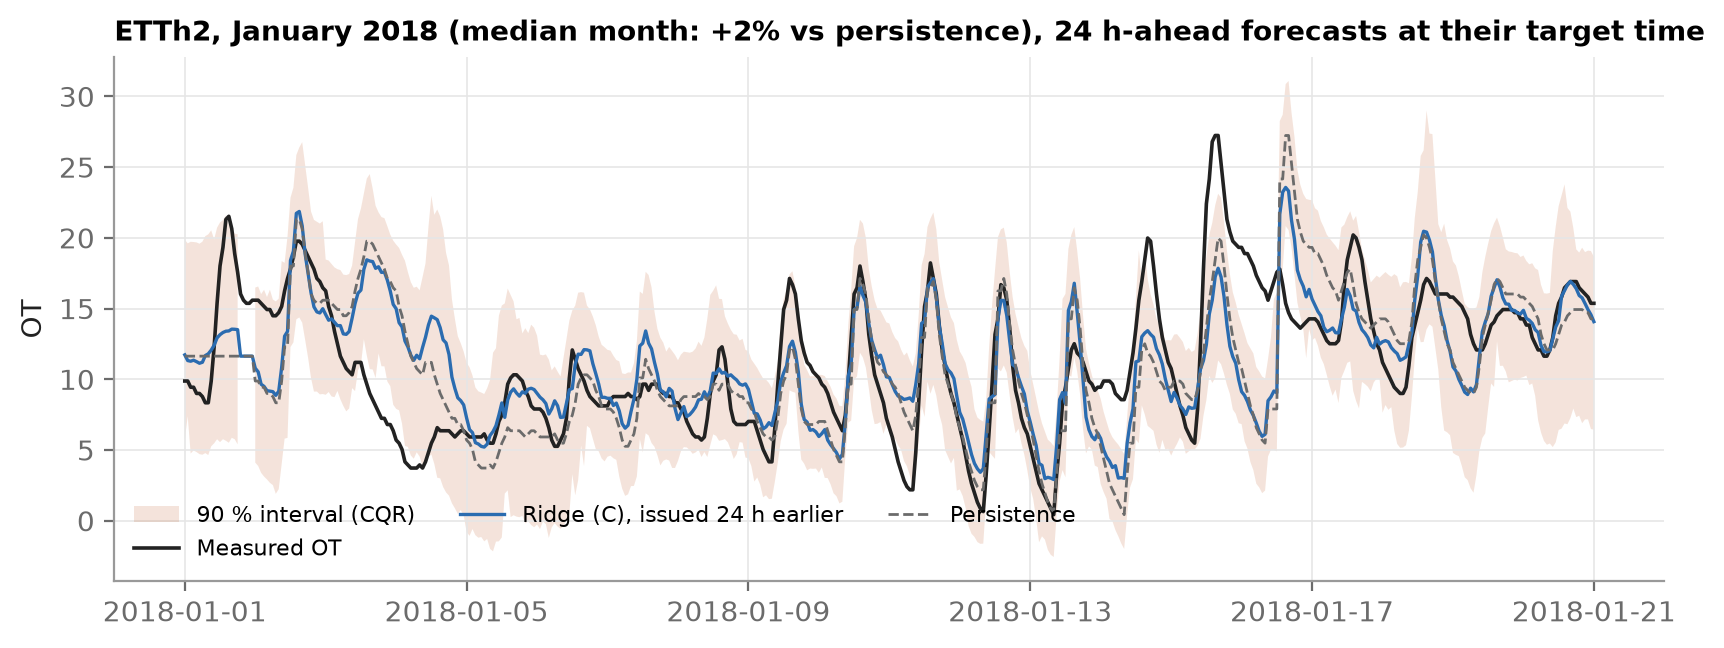
\includegraphics[width=\textwidth]{res_example_forecast}
    \end{column}
    \begin{column}{0.36\textwidth}
      \footnotesize
      \renewcommand{\arraystretch}{1.25}
      \begin{tabular}{l c c}
        \toprule
        & 補正前 & \textbf{CQR後} \\
        \midrule
        被覆率 ETTh1 & 84\% & \hlg{90\%} \\
        被覆率 ETTh2 & 77\% & \hlg{90\%} \\
        区間幅 ETTh1 & 6.0℃ & 7.2℃ \\
        区間幅 ETTh2 & 9.3℃ & 12.7℃ \\
        \bottomrule
      \end{tabular}
      \vspace{0.2cm}
      \begin{itemize}\setlength{\itemsep}{2pt}
        \item 名目どおりの信頼度を\hl{実測で確認}してから保全判断に使うべき
        \item 区間が広い（ETTh2で約±6℃）のは外気温不在による本質的な不確実性
      \end{itemize}
    \end{column}
  \end{columns}
  \source{CQR：Romano et al. (2019)。各分割で直近60日を校正用に確保。数値は計画あり（C）。}
\end{frame}

% ------------------------------------------------------------------ 13 robustness
\settag{業務価値 ③ 負荷計画の品質条件}
\begin{frame}{負荷計画の誤差が10\%程度までなら効果は残るが、20\%では両変電所とも計画なし予測を下回るため、計画精度が導入条件となる}
  \begin{columns}[T]
    \begin{column}{0.55\textwidth}
      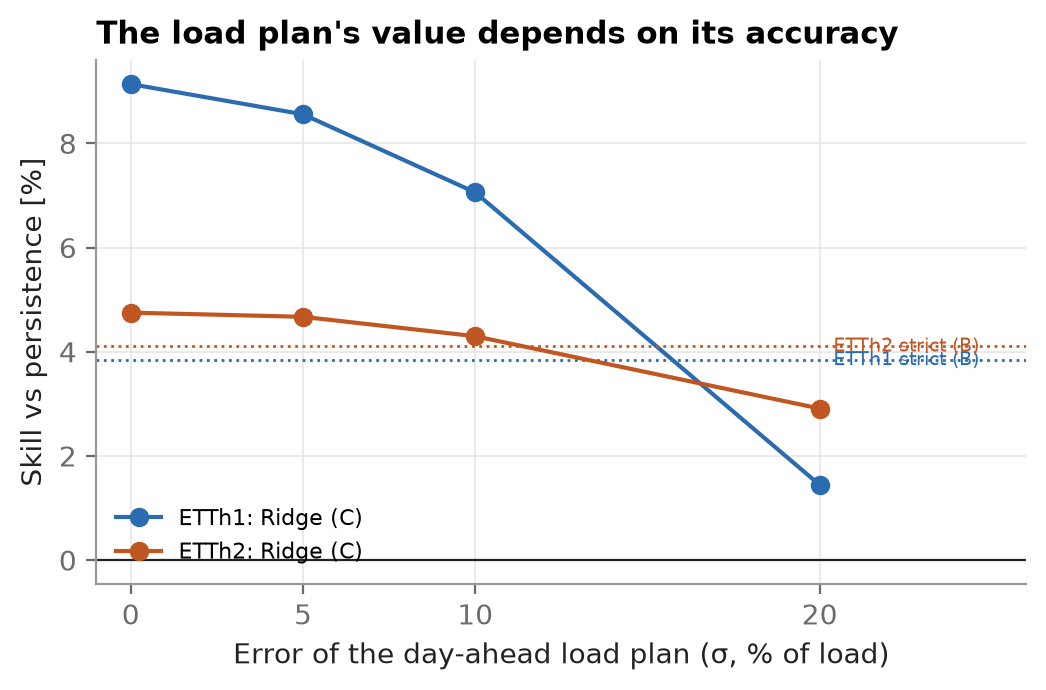
\includegraphics[width=\textwidth]{res_load_noise}
    \end{column}
    \begin{column}{0.43\textwidth}
      \footnotesize
      \begin{itemize}\setlength{\itemsep}{3pt}
        \item 実負荷に日次バイアス＋時間ノイズ（σ）を加えて「不完全な計画」を模擬
        \item ETTh1：スキル 9.1\%（誤差0）→ 7.1\%（10\%）→ \hlb{1.4\%（20\%）}。計画なし（3.8\%）を下回る
        \item ETTh2：4.8\% → 4.3\% → \hlb{2.9\%（20\%）}。計画なし（4.1\%）を下回る
        \item \hl{要件}：日前負荷計画の誤差がおおむね10\%以内であること。満たせない場合は計画なし（B）で運用
      \end{itemize}
    \end{column}
  \end{columns}
  \source{学習時は真の負荷を使用し、評価時のみ計画誤差を付与（運用時の状況を再現）。モデル：Ridge（C）。}
\end{frame}

% ------------------------------------------------------------------ 14 failure analysis
\settag{課題分析}
\begin{frame}{誤差は季節の変わり目と高温時に集中し、ETTh2の最高温域ではモデルが「現在値維持」より誤差が大きい}
  \centering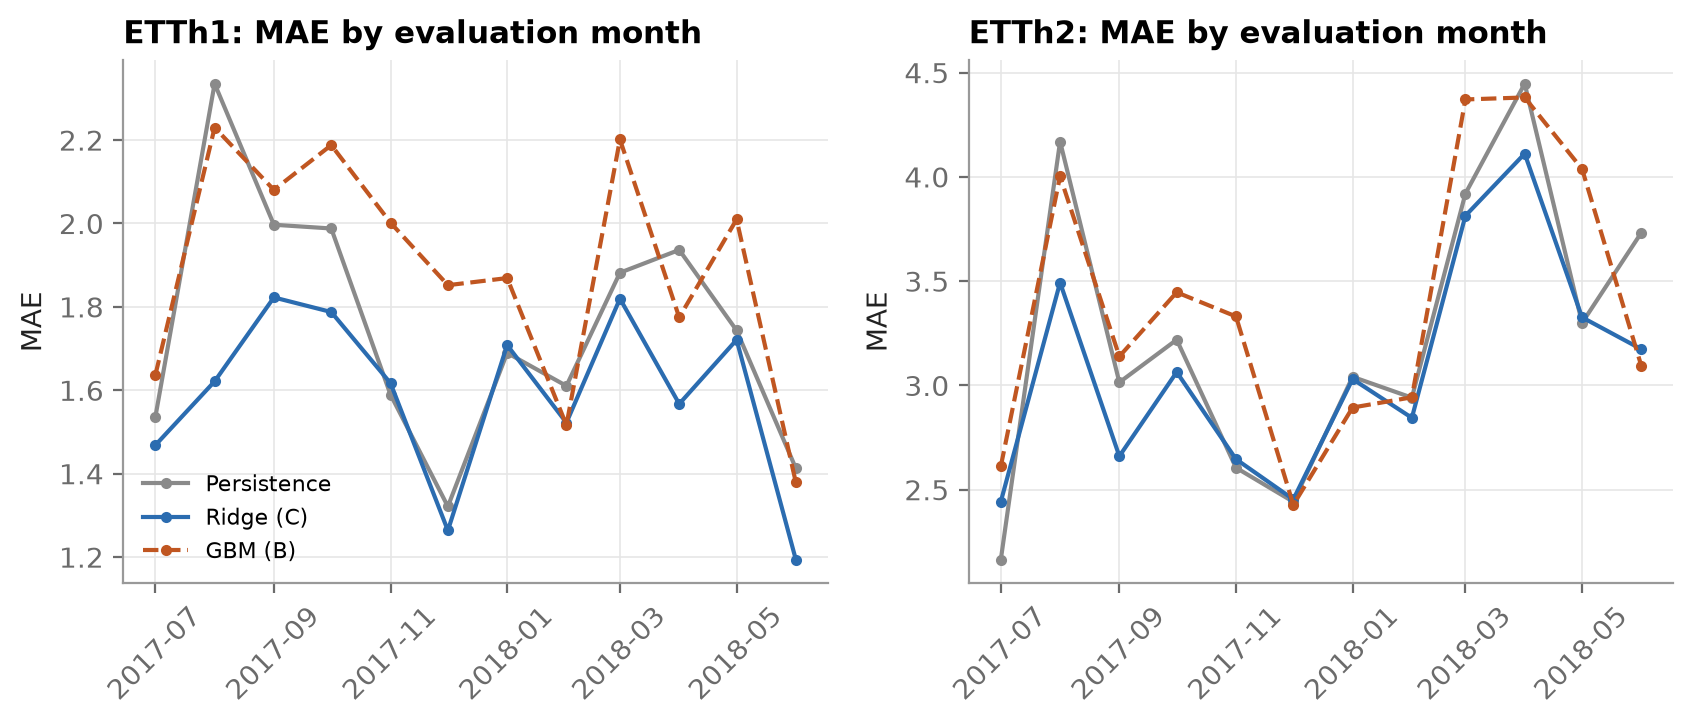
\includegraphics[width=\textwidth,height=4.1cm,keepaspectratio]{res_monthly}\par\raggedright
  \footnotesize
  \begin{itemize}\setlength{\itemsep}{1pt}
    \item 高温時（開発期間の上位10\%）のMAE（ETTh2）：現在値維持 \textbf{2.69℃} に対し Ridge（C）3.07℃、ピーク重視GBM 3.10℃。\hlb{ピークを平均側へ引き戻す傾向}
    \item 唯一LSTM（B）が2.56℃と下回り、系列モデルは極値で有望。高温域専用モデルや外気温の追加で改善余地
    \item 警告では余裕幅でこの過小予測を補っている（p.12）
  \end{itemize}
\end{frame}

% ------------------------------------------------------------------ 15 anomaly
\settag{発展 ① 異常検知}
\begin{frame}{データ品質監視は即日導入できるが、「期待油温との差」による冷却異常検知は外気温なしでは実用水準に届かない}
  \begin{columns}[T]
    \begin{column}{0.49\textwidth}
      \softbox{}{\footnotesize\textbf{ルールベースのデータ品質監視：有効}
      \begin{itemize}\setlength{\itemsep}{1pt}
        \item 固着・スパイク・31日凍結・負荷バランス崩れを過去データのみで検知
        \item 本データで実際に\hl{43日間の固着}等を発見（p.4）
        \item 検知時は予測を安全側（現在値維持）に切替
      \end{itemize}}
    \end{column}
    \begin{column}{0.49\textwidth}
      \softbox{}{\footnotesize\textbf{モデル残差による冷却異常検知：未達}
      \begin{itemize}\setlength{\itemsep}{1pt}
        \item 負荷から期待油温を推定し、6時間平均の差で警報（Djamali \& Tenbohlen、CIGREのデジタルツイン方式）
        \item 擬似故障（+3〜8℃）の検知率は\hlb{10\%以下}。期待値モデルが故障を「追従」してしまい、差が警報閾値（正常時の99.5\%点：1.5〜1.7℃）に届かない
        \item 12時間で+20℃の急変はETTh1で全件検知（ETTh2は10\%）
      \end{itemize}}
    \end{column}
  \end{columns}
  \vspace{0.2cm}
  \footnotesize
  \textbf{結論}：異常検知は「外気温」と「冷却装置の運転状態」を入力に加えて再評価すべき。現状データで導入するのはデータ品質監視に限定する。
  \source{擬似故障：12時間で線形上昇しその後36時間維持、各条件30件。閾値は開発期間の正常窓における99.5パーセンタイル。}
\end{frame}

% ------------------------------------------------------------------ 16 limitations
\settag{現時点の限界}
\begin{frame}{本PoCは公開データでの技術的な見込みを示したに過ぎず、実設備での有効性は外気温・実警報値・故障履歴で確認する必要がある}
  \footnotesize
  \renewcommand{\arraystretch}{1.35}
  \begin{tabularx}{\textwidth}{>{\bfseries}p{3.4cm} X X}
    \toprule
    限界 & 影響 & 解消に必要なもの \\
    \midrule
    外気温データなし & 日内変動の主因を説明できず、精度と異常検知の上限を規定 & 最寄り気象観測点の時別気温（設置場所の情報） \\
    実警報値・故障履歴なし & 代理警報値での評価に留まり、業務価値（回避損失）を金額換算できない & 運用中の警報設定、過去の保全記録 \\
    評価イベントが少ない & 過熱開始15件のみ。警告率の不確実性が大きい & 変圧器・期間の追加 \\
    変圧器2台のみ & 他設備への汎化は未検証。2台で挙動（時定数・品質）が大きく異なる & 設備台帳（冷却方式・定格）と複数台データ \\
    負荷計画は模擬 & 実計画の精度・入手時刻は未確認 & 実際の日前計画データ \\
    \bottomrule
  \end{tabularx}
\end{frame}

% ------------------------------------------------------------------ 17 next steps
\settag{今後の進め方}
\begin{frame}{外気温の追加と3か月のシャドー運用を経て、合格基準を満たせば予測アラートを本導入することを提案する}
  \centering
  \begin{tikzpicture}[font=\scriptsize, node distance=0.35cm,
      stepbox/.style={draw=accent, thick, fill=soft, rounded corners=2pt, text width=4.1cm, minimum height=2.9cm, align=left, inner sep=5pt}]
    \node[stepbox] (a) {\textbf{\color{accent}Step 1（1か月）\\データ拡充}\\[3pt]
      ・外気温（気象データ）を連携\\・実警報値・保全記録の共有\\・データ品質監視を先行導入\\[3pt]
      \textbf{合格基準}：外気温追加でMAEが現状比10\%以上改善};
    \node[stepbox, right=of a] (b) {\textbf{\color{accent}Step 2（3か月）\\シャドー運用}\\[3pt]
      ・予測と警告を運用画面に並行表示（判断には使わない）\\・誤報・見逃しを記録\\[3pt]
      \textbf{合格基準}：過熱の80\%以上を12時間前までに警告、誤報は月10件以下};
    \node[stepbox, right=of b] (c) {\textbf{\color{accent}Step 3\\本導入・拡大}\\[3pt]
      ・警告ルールを保全手順に組込\\・異常検知（冷却系）を再評価\\・対象変圧器を拡大\\[3pt]
      \textbf{継続監視}：月次で被覆率・誤差・ドリフトを確認、再学習};
    \draw[->,thick,accent] (a) -- (b);
    \draw[->,thick,accent] (b) -- (c);
  \end{tikzpicture}
  \vspace{0.3cm}
  \footnotesize
  \begin{itemize}
    \item 本PoCのコード（データ品質判定・特徴量・ロール検証・区間校正・警告シミュレーション）はそのまま Step 2 の評価基盤として再利用できる
  \end{itemize}
\end{frame}

% ------------------------------------------------------------------ appendix
\settag{付録 A　比較したモデル}
\begin{frame}{付録：比較したモデルと設定}
  \scriptsize
  \renewcommand{\arraystretch}{1.2}
  \begin{tabularx}{\textwidth}{>{\bfseries}p{3.2cm} X}
    \toprule
    モデル & 内容 \\
    \midrule
    現在値維持／24h移動平均 & 基準。24h先では「前日同時刻」と同一 \\
    グレーボックス熱モデル & IEC 60076-7の一次遅れモデルを離散化。時定数τ（推定36〜48h）と負荷係数を学習。外気温は季節・時刻の調和関数と週平均油温で代用 \\
    Ridge & 物理特徴量（S²、S²の指数平滑3/12/48h、油温変化、カレンダー）。正則化係数は開発期間で選択 \\
    GBM／頑健化／ピーク重視 & HistGradientBoosting。頑健化：油温水準を除外し直近データを重視（半減期180日）。ピーク重視：上位10\%を3倍重み \\
    ハイブリッド & グレーボックスの残差をGBMで学習 \\
    MLP／LSTM & MLP（64-32）。LSTM：過去72時間の生系列＋（C）翌24時間の計画、早期終了 \\
    生ウィンドウ線形 & 過去168時間の油温・S²（＋計画24時間）にRidge（DLinear型） \\
    アンサンブル／+BC & Ridge・頑健化GBM・ハイブリッドの等重み平均。+BC：直近7日の誤差平均を差し引く \\
    CQR & 分位点GBM（5\%・95\%）＋コンフォーマル補正 \\
    \bottomrule
  \end{tabularx}
\end{frame}

\settag{付録 B　参考文献}
\begin{frame}{付録：参考文献}
  \tiny
  \begin{enumerate}\setlength{\itemsep}{0pt}
    \item H. Zhou et al. Informer: Beyond Efficient Transformer for Long Sequence Time-Series Forecasting. AAAI 2021.（ETTデータセット, CC BY-ND 4.0）
    \item IEC 60076-7:2018 Loading guide for mineral-oil-immersed power transformers. ／ IEEE Std C57.91-2011.
    \item D. Tembo et al. Data-Driven vs Traditional Approaches to Power Transformer's Top-Oil Temperature Estimation. arXiv:2501.16831, 2025.
    \item M. Djamali, S. Tenbohlen. Malfunction Detection of the Cooling System in Air-Forced Power Transformers Using Online Thermal Monitoring. IEEE Trans. Power Delivery, 2017.
    \item CIGRE. Digital twins for power transformers: concept and future perspectives. Electra, 2026.
    \item H. Hewamalage, K. Ackermann, C. Bergmeir. Forecast evaluation for data scientists: common pitfalls and best practices. Data Min. Knowl. Disc. 37, 2023.
    \item Y. Cui, J. Xie, K. Zheng. Historical Inertia: A Neglected but Powerful Baseline for Long Sequence Time-Series Forecasting. CIKM 2021.
    \item A. Zeng et al. Are Transformers Effective for Time Series Forecasting? AAAI 2023.
    \item F. X. Diebold, R. S. Mariano. Comparing Predictive Accuracy. JBES, 1995. ／ D. Harvey, S. Leybourne, P. Newbold. IJF, 1997.
    \item L. Tashman. Out-of-sample tests of forecasting accuracy. IJF, 2000.
    \item T. Januschowski et al. Forecasting with trees. IJF, 2022.
    \item J. Smith, K. F. Wallis. A Simple Explanation of the Forecast Combination Puzzle. Oxford Bull. Econ. Stat., 2009.
    \item Y. Romano, E. Patterson, E. Candès. Conformalized Quantile Regression. NeurIPS 2019.
  \end{enumerate}
  \vspace{0.2cm}
  {\scriptsize\color{muted}実装・全結果：GitHub リポジトリ（README に再現手順）}
\end{frame}

\end{document}
